% VerdeAI gap-analysis pipeline — research-paper figure (v6: slot-filling +
% coverage/critical-slot decision scoring).
%
% Standalone file: compiles on its own (e.g. on Overleaf) to a single
% cropped PDF/PNG you can \includegraphics{} directly.
%
% To embed inside an existing paper instead of using it standalone:
%   1. Copy everything from \begin{tikzpicture} to \end{tikzpicture}.
%   2. Paste it inside your own:
%        \begin{figure*}[t]
%          \centering
%          <paste tikzpicture here>
%          \caption{VerdeAI's document-to-gap-report pipeline. Ingestion
%            (top row) indexes uploaded evidence once; per-clause gap
%            analysis (middle two rows) then answers a fixed slot schema
%            per ISO~14001 clause and derives a decision arithmetically
%            from slot coverage, rather than trusting a free-text LLM
%            verdict. Shapes follow standard flowchart convention:
%            input/output, decision, deterministic process, model-call
%            (``predefined process''), and document output.}
%          \label{fig:verdeai-pipeline}
%        \end{figure*}
%   3. Copy the \usetikzlibrary{...} line and the \definecolor / \tikzset
%      blocks into your own preamble (or a shared style file).
%
% The diagram is wide and four rows tall. In a two-column paper, scale it
% to fit rather than shrinking font size, e.g.:
%   \resizebox{\linewidth}{!}{\includegraphics{verdeai-pipeline-figure}}
%
\documentclass[tikz, border=6mm]{standalone}
\usetikzlibrary{shapes.geometric, arrows.meta, positioning, calc}

% ---- palette: muted, print-safe. One hue per SHAPE CATEGORY (not per
% step), so the legend maps directly onto the shape vocabulary and the
% figure still reads correctly if printed in grayscale (shape carries
% the meaning; color is a redundant, secondary cue). ----
\definecolor{inkcolor}{HTML}{17241B}     % borders + text
\definecolor{mutedtext}{HTML}{4D5D4F}    % secondary/caption text
\definecolor{terminalfill}{HTML}{F2F3EF} % start / end
\definecolor{iofill}{HTML}{B7C6DA}       % input / output (parallelogram)
\definecolor{decisionfill}{HTML}{E6D3A3} % decision (diamond)
\definecolor{processfill}{HTML}{BFD3BC}  % deterministic process (rectangle)
\definecolor{aifill}{HTML}{CBB9D6}       % AI / model call (predefined process)
\definecolor{reportfill}{HTML}{3E5C43}   % final report (document shape)
\definecolor{abstainfill}{HTML}{D9CBB8}  % abstain / insufficient-evidence output

\begin{document}
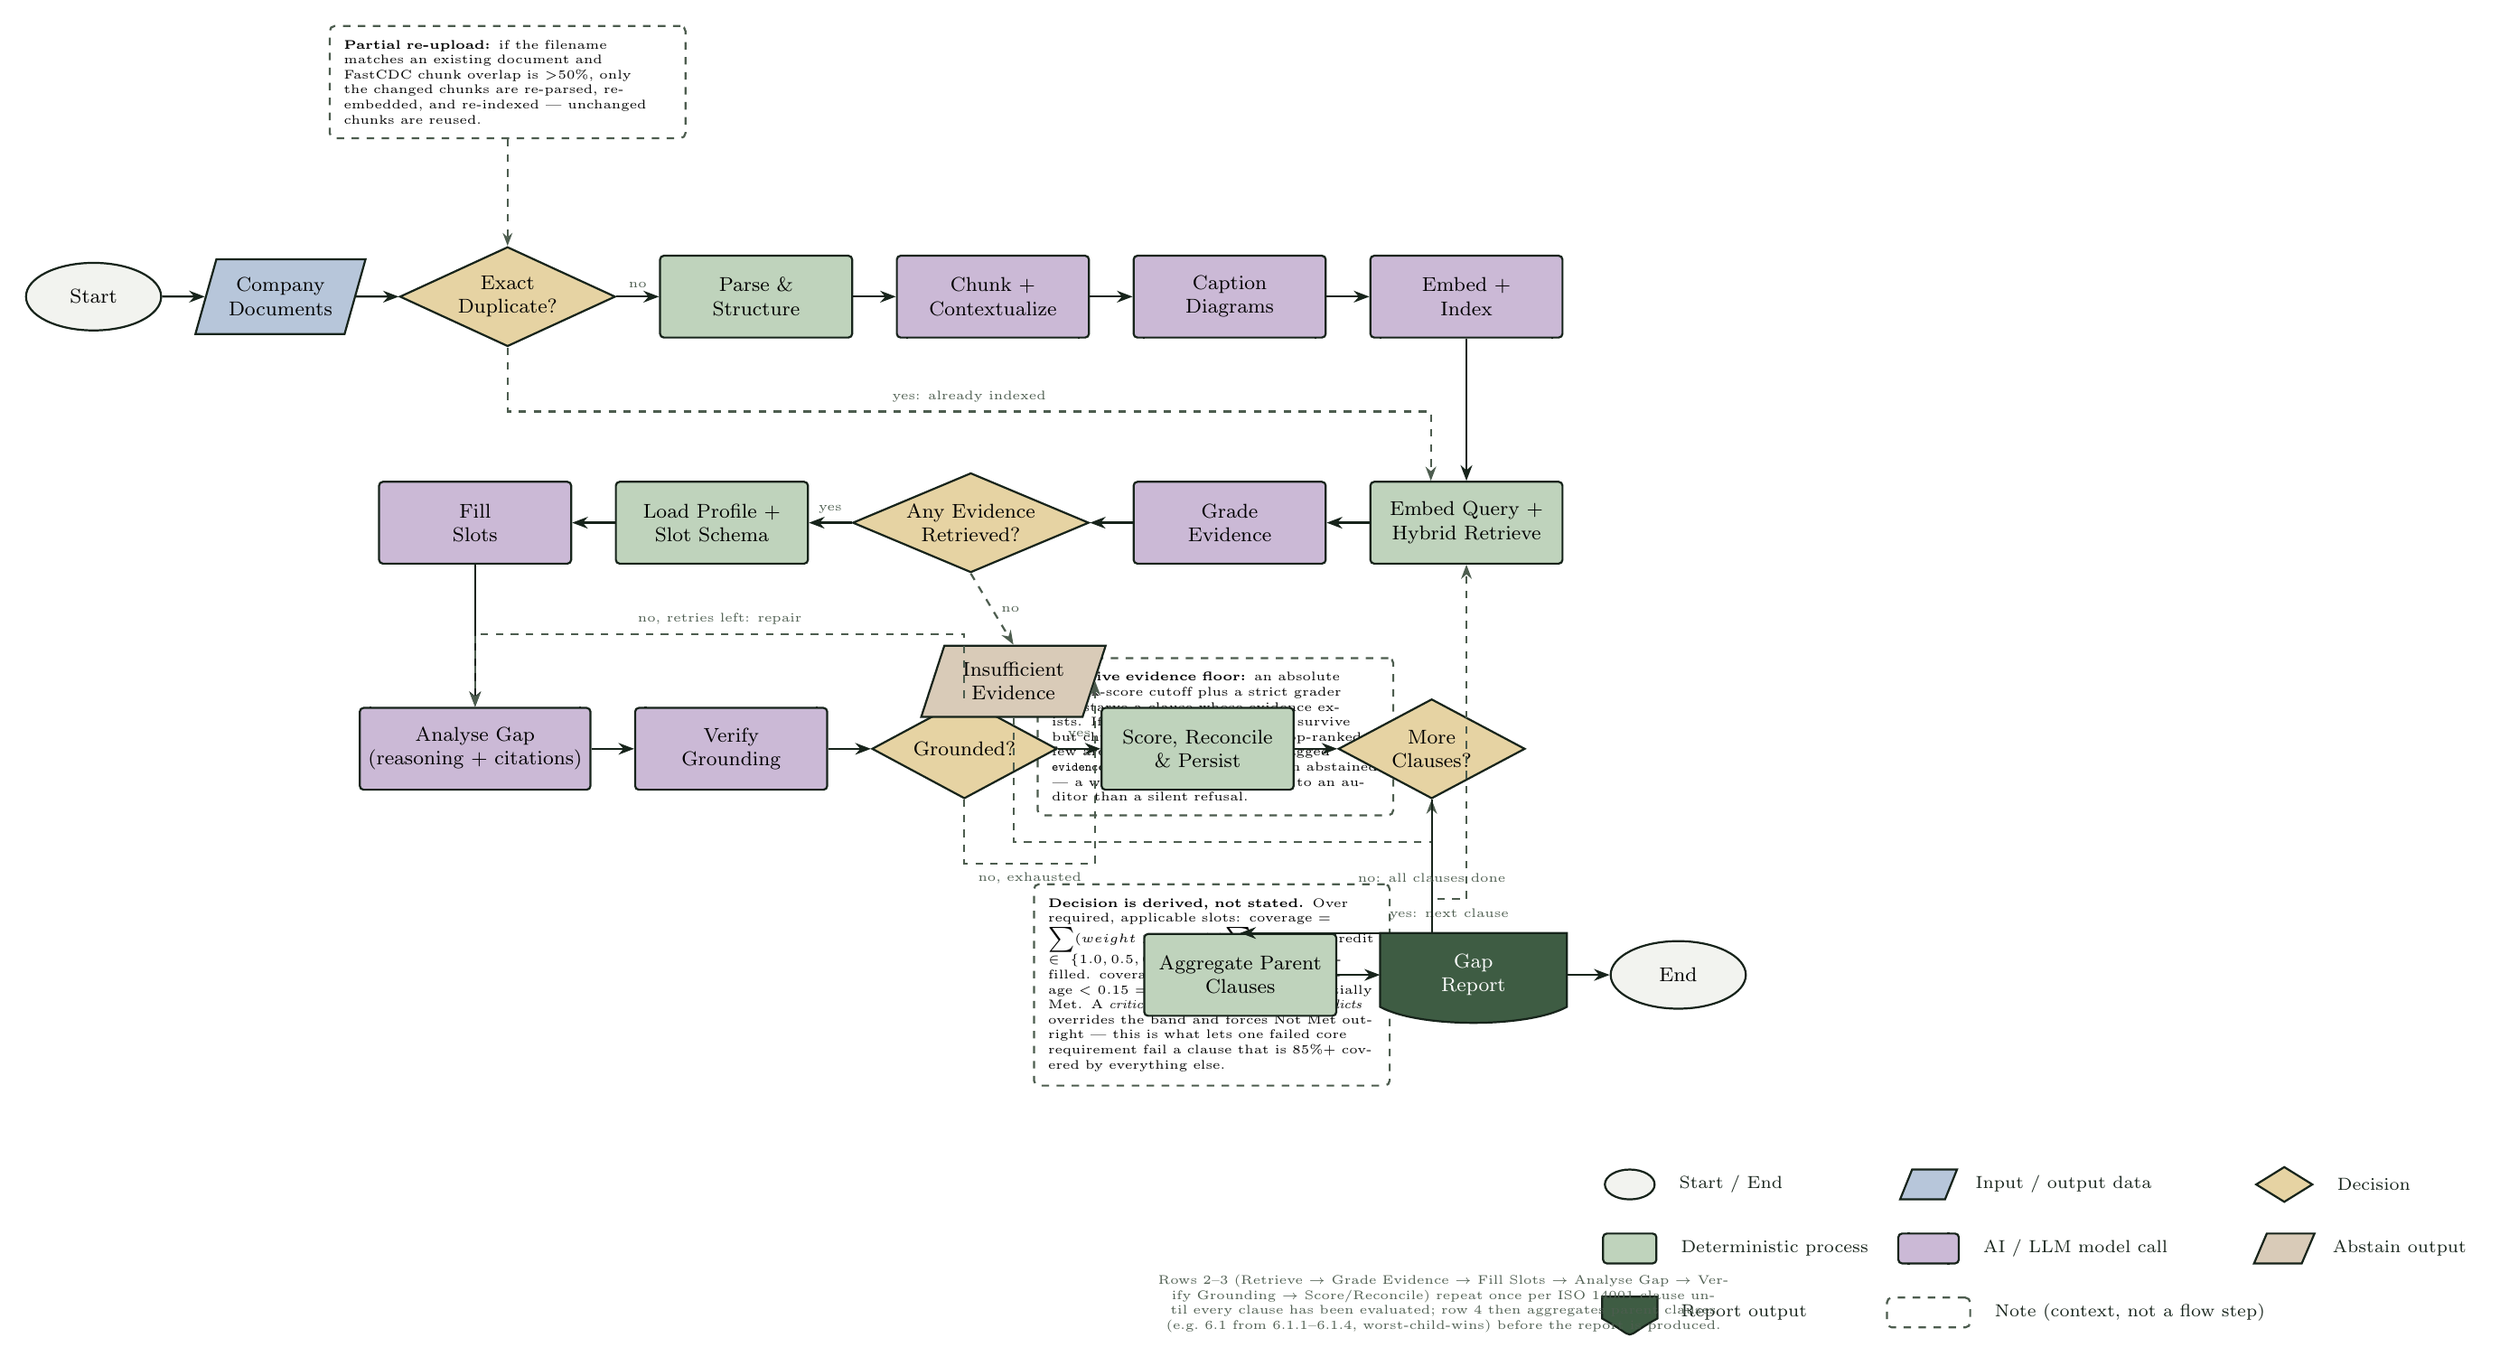
\begin{tikzpicture}[
  >=Stealth,
  every node/.style={font=\footnotesize},
  node distance=6mm and 6mm,
  align=center,
  thick,
]

% ---------------------------------------------------------------
% Node style vocabulary — one style per flowchart meaning.
% ---------------------------------------------------------------
\tikzset{
  terminal/.style={
    ellipse, draw=inkcolor, fill=terminalfill,
    minimum width=1.9cm, minimum height=0.95cm,
  },
  io/.style={
    trapezium, trapezium left angle=70, trapezium right angle=110,
    trapezium stretches=true,
    draw=inkcolor, fill=iofill,
    minimum width=2.4cm, minimum height=1.05cm,
  },
  abstain/.style={
    trapezium, trapezium left angle=70, trapezium right angle=110,
    trapezium stretches=true,
    draw=inkcolor, fill=abstainfill,
    minimum width=2.6cm, minimum height=1.0cm,
  },
  decision/.style={
    diamond, draw=inkcolor, fill=decisionfill, aspect=2.4,
    inner sep=1pt, minimum width=2.6cm, minimum height=1.4cm,
  },
  process/.style={
    rectangle, rounded corners=1.5pt, draw=inkcolor, fill=processfill,
    minimum width=2.7cm, minimum height=1.15cm,
  },
  subprocess/.style={
    rectangle, rounded corners=1.5pt, draw=inkcolor, fill=aifill,
    minimum width=2.7cm, minimum height=1.15cm,
    append after command={
      \pgfextra{
        \draw[inkcolor]
          ($(\tikzlastnode.north west)!0.16cm!(\tikzlastnode.north east)$)
          -- ($(\tikzlastnode.south west)!0.16cm!(\tikzlastnode.south east)$);
        \draw[inkcolor]
          ($(\tikzlastnode.north east)!0.16cm!(\tikzlastnode.north west)$)
          -- ($(\tikzlastnode.south east)!0.16cm!(\tikzlastnode.south west)$);
      }
    },
  },
  flowline/.style={-{Stealth[length=2.2mm]}, inkcolor},
  branchline/.style={-{Stealth[length=2mm]}, mutedtext, dashed},
  annotation/.style={
    rectangle, rounded corners=2pt, draw=mutedtext, dashed, fill=white,
    text width=4.6cm, font=\tiny, align=left, inner sep=2mm,
  },
}

% Draws a hand-built "document" symbol (rectangle with a wavy bottom
% edge) at the position/size of an existing (invisible) node #1, with
% label text #2. Used instead of a named shape library so the file has
% no dependency beyond shapes.geometric.
\newcommand{\documentshape}[2]{
  \draw[inkcolor, fill=reportfill]
    (#1.north west) -- (#1.north east)
    -- ($(#1.south east)+(0,0.14)$)
    .. controls ($(#1.south east)+(-0.55,-0.16)$) and ($(#1.south west)+(0.55,-0.16)$) ..
    ($(#1.south west)+(0,0.14)$) -- cycle;
  \node[text=white, align=center] at (#1) {#2};
}

% =================================================================
% ROW 1 — document ingestion & indexing (services/document-processor,
% stages 1-6: dedup, parse, chunk+contextualize, caption, embed, index).
% Left to right.
% =================================================================
\node[terminal]                              (start)    {Start};
\node[io,         right=of start]            (docs)     {Company\\Documents};
\node[decision,   right=of docs]             (dup)      {Exact\\Duplicate?};
\node[process,    right=of dup]              (parse)    {Parse \&\\Structure};
\node[subprocess, right=of parse]            (chunk)    {Chunk +\\Contextualize};
\node[subprocess, right=of chunk]            (caption)  {Caption\\Diagrams};
\node[subprocess, right=of caption]          (embed)    {Embed +\\Index};

\node[annotation, above=15mm of dup] (note1)
  {\textbf{Partial re-upload:} if the filename matches an existing
  document and FastCDC chunk overlap is $>$50\%, only the changed
  chunks are re-parsed, re-embedded, and re-indexed --- unchanged
  chunks are reused.};
\draw[mutedtext, dashed, -{Stealth[length=1.8mm]}] (note1.south) -- (dup.north);

% =================================================================
% ROW 2 — retrieval & evidence sufficiency, per ISO 14001 clause
% (services/gap-analyzer/app/pipeline/analyse_clause.py:
%  embed -> retrieve -> grade_evidence -> [route_after_grade]
%  -> load_org_profile -> load_slot_schema -> slot_fill).
% Right to left, directly below row 1.
% =================================================================
\node[process,    below=20mm of embed]       (retrieve) {Embed Query +\\Hybrid Retrieve};
\node[subprocess, left=of retrieve]          (grade)    {Grade\\Evidence};
\node[decision,   left=of grade]             (haseve)   {Any Evidence\\Retrieved?};
\node[process,    left=of haseve]            (loadctx)  {Load Profile +\\Slot Schema};
\node[subprocess, left=of loadctx]           (fill)     {Fill\\Slots};

\node[annotation, below=13mm of grade, xshift=-2mm] (note2)
  {\textbf{Relative evidence floor:} an absolute rerank-score cutoff
  plus a strict grader can starve a clause whose evidence exists.
  If fewer than the minimum survive but chunks \emph{were} retrieved,
  the top-ranked few are kept and the result is flagged
  \texttt{evidence\_status=degraded} rather than abstained --- a weak
  answer is more useful to an auditor than a silent refusal.};

% =================================================================
% ROW 3 — LLM judgement, grounding verification, and the deterministic
% decision (gap_analyse -> verify_grounding -> [route_after_verify]
% -> reconcile/persist, then the per-clause loop -> reconcile).
% Left to right, directly below row 2.
% =================================================================
\node[subprocess, below=20mm of fill]        (analyse)  {Analyse Gap\\(reasoning + citations)};
\node[subprocess, right=of analyse]          (verify)   {Verify\\Grounding};
\node[decision,   right=of verify]           (grounded) {Grounded?};
\node[process,    right=of grounded]         (score)    {Score, Reconcile\\\& Persist};
\node[decision,   right=of score]            (more)     {More\\Clauses?};

\node[abstain, below=10mm of haseve, xshift=6mm] (insuff) {Insufficient\\Evidence};

\node[annotation, below=13mm of score, xshift=2mm] (note3)
  {\textbf{Decision is derived, not stated.} Over required, applicable
  slots: coverage $=\sum(\text{weight}\times\text{credit})/\sum(\text{weight})$,
  credit $\in\{1.0,0.5,0.0\}$ for filled/partial/not-filled.
  coverage~$\geq 0.85\Rightarrow$~Met; coverage~$<0.15\Rightarrow$~Not Met;
  otherwise Partially Met. A \emph{critical} slot the evidence
  \emph{contradicts} overrides the band and forces Not Met outright ---
  this is what lets one failed core requirement fail a clause that is
  85\%+ covered by everything else.};

% =================================================================
% ROW 4 — once per analysis, after every clause has been visited:
% deterministic parent-clause aggregation, then the report.
% =================================================================
\node[process,    below=20mm of score, xshift=6mm]  (aggregate) {Aggregate Parent\\Clauses};
\node[rectangle, minimum width=2.6cm, minimum height=1.15cm,
      right=of aggregate]                            (reportbox) {};
\node[terminal,   right=of reportbox]                (end)      {End};

% =================================================================
% Main flow — row 1
% =================================================================
\draw[flowline] (start) -- (docs);
\draw[flowline] (docs) -- (dup);
\draw[flowline] (dup) -- node[above, font=\tiny, text=mutedtext]{no} (parse);
\draw[flowline] (parse) -- (chunk);
\draw[flowline] (chunk) -- (caption);
\draw[flowline] (caption) -- (embed);

% bend: row 1 -> row 2 (first pass over a clause)
\draw[flowline] (embed.south) -- (retrieve.north);

% Main flow — row 2 (right to left)
\draw[flowline] (retrieve) -- (grade);
\draw[flowline] (grade) -- (haseve);
\draw[flowline] (haseve) -- node[above, font=\tiny, text=mutedtext]{yes} (loadctx);
\draw[flowline] (loadctx) -- (fill);

% bend: row 2 -> row 3
\draw[flowline] (fill.south) -- (analyse.north);

% Main flow — row 3 (left to right)
\draw[flowline] (analyse) -- (verify);
\draw[flowline] (verify) -- (grounded);
\draw[flowline] (grounded) -- node[above, font=\tiny, text=mutedtext]{yes} (score);
\draw[flowline] (score) -- (more);

% Main flow — row 4
\draw[flowline] (aggregate) -- (reportbox);
\draw[flowline] (reportbox) -- (end);

% =================================================================
% Branch 1 — duplicate short-circuit: skip straight to retrieval,
% the document's chunks are already indexed from a prior upload.
% =================================================================
\coordinate (bypassLane)  at ($(dup.south)+(0,-0.9)$);
\coordinate (bypassEntry) at ($(retrieve.north)+(-0.5,0)$);
\coordinate (bypassTurn)  at (bypassEntry |- bypassLane);
\draw[branchline]
  (dup.south) -- (bypassLane)
  -- node[above, font=\tiny, text=mutedtext]{yes: already indexed} (bypassTurn)
  -- (bypassEntry);

% =================================================================
% Branch 2 — evidence grading found nothing retrieved at all: abstain.
% (The "degraded" case, by contrast, still flows through the
% "yes" edge above with a flag on the result — see note2.)
% =================================================================
\draw[branchline] (haseve.south) -- node[right, font=\tiny, text=mutedtext]{no} (insuff.north);

% =================================================================
% Branch 3 — bounded grounding-repair loop: an ungrounded verdict
% (fabricated citation, missing evidence for the decision) is sent
% back to "Analyse Gap" with feedback, up to MAX_VERIFY_RETRIES times.
% =================================================================
\coordinate (repairLane) at ($(grounded.north)+(0,0.9)$);
\coordinate (repairTurn) at (analyse.north |- repairLane);
\draw[branchline]
  (grounded.north) -- (repairLane)
  -- node[above, font=\tiny, text=mutedtext]{no, retries left: repair} (repairTurn)
  -- (analyse.north);

% =================================================================
% Branch 4 — grounding retries exhausted: abstain to Insufficient
% Evidence rather than persist an ungrounded verdict.
% =================================================================
\coordinate (giveupLane) at ($(grounded.south)+(0,-0.9)$);
\coordinate (giveupTurn) at (insuff.east |- giveupLane);
\draw[branchline]
  (grounded.south) -- (giveupLane)
  -- node[below, font=\tiny, text=mutedtext]{no, exhausted} (giveupTurn)
  -- (insuff.east);

% Insufficient Evidence still counts as this clause's persisted result,
% so it re-joins the loop check exactly like a scored verdict does.
\draw[branchline] (insuff.south) |- ($(more.south)+(0,-0.6)$) -| (more.south);

% =================================================================
% Branch 5 — loop back for the next ISO 14001 clause, re-entering
% row 2's retrieval step from below.
% =================================================================
\coordinate (loopLane)  at ($(more.south)+(0,-1.4)$);
\coordinate (loopEntry) at (retrieve.south);
\coordinate (loopTurn)  at (loopEntry |- loopLane);
\draw[branchline]
  (more.south) -- (loopLane)
  -- node[below, font=\tiny, text=mutedtext]{yes: next clause} (loopTurn)
  -- (loopEntry);

% "More clauses? no" -> once-per-analysis aggregation step.
\draw[flowline] (more.south) -- ++(0,-0.7) coordinate (moreDrop)
  |- node[near start, above, font=\tiny, text=mutedtext]{no: all clauses done} (aggregate.north);

% document (report) shape, drawn on top of its placeholder node
\documentshape{reportbox}{Gap\\Report}

% =================================================================
% Legend — placed below the whole diagram.
% =================================================================
\begin{scope}[shift={($(end.south west)+(0,-2.6)$)}]
  \node[terminal, minimum width=0.7cm, minimum height=0.42cm, font=\tiny] (l1) at (0,0) {};
  \node[right=2mm of l1, font=\scriptsize, text=inkcolor] {Start / End};

  \node[io, minimum width=0.8cm, minimum height=0.42cm, font=\tiny] (l2) at (4.2,0) {};
  \node[right=2mm of l2, font=\scriptsize, text=inkcolor] {Input / output data};

  \node[decision, minimum width=0.8cm, minimum height=0.5cm, font=\tiny] (l3) at (9.2,0) {};
  \node[right=2mm of l3, font=\scriptsize, text=inkcolor] {Decision};

  \node[process, minimum width=0.75cm, minimum height=0.42cm, font=\tiny] (l4) at (0,-0.9) {};
  \node[right=2mm of l4, font=\scriptsize, text=inkcolor] {Deterministic process};

  \node[subprocess, minimum width=0.85cm, minimum height=0.42cm, font=\tiny] (l5) at (4.2,-0.9) {};
  \node[right=2mm of l5, font=\scriptsize, text=inkcolor] {AI / LLM model call};

  \node[abstain, minimum width=0.85cm, minimum height=0.42cm, font=\tiny] (l6) at (9.2,-0.9) {};
  \node[right=2mm of l6, font=\scriptsize, text=inkcolor] {Abstain output};

  \node[rectangle, minimum width=0.75cm, minimum height=0.42cm] (l7) at (0,-1.8) {};
  \documentshape{l7}{}
  \node[right=2mm of l7, font=\scriptsize, text=inkcolor] {Report output};

  \node[annotation, text width=1.1cm, minimum height=0.42cm, inner sep=1pt,
        font=\tiny] (l8) at (4.2,-1.8) {};
  \node[right=2mm of l8, font=\scriptsize, text=inkcolor] {Note (context, not a flow step)};
\end{scope}

\node[font=\tiny, text=mutedtext, below=6mm of end, xshift=-3.3cm, yshift=-3.0cm, text width=9cm, align=center]
  {Rows 2--3 (Retrieve $\rightarrow$ Grade Evidence $\rightarrow$ Fill Slots $\rightarrow$
  Analyse Gap $\rightarrow$ Verify Grounding $\rightarrow$ Score/Reconcile) repeat once per
  ISO~14001 clause until every clause has been evaluated; row~4 then aggregates parent
  clauses (e.g.\ 6.1 from 6.1.1--6.1.4, worst-child-wins) before the report is produced.};

\end{tikzpicture}
\end{document}
